\section{Common Algorithms}

\subsection{Noise Generation}
\label{section:noise-generation}
Nature's unpredictability and plays a big role in the diversity and appearance of cloudscapes. In shaders, an approach to that \textit{randomness} is used called \textit{\gls{noise}}.
In order to be able to implement random \gls{noise}, several important topics need to be looked into. It is best to start with randomness in computer science and how it is handled inside a shader program.

\subsubsection{Random Numbers}
As expected, there is no magic function which returns a pure random number inside the seemingly predictable and rigid code environment.
So the question how to generate randomness arises. 
\\
For this, the function $rnd(x) = fract(sin(x))$ is inspected, where $fract(x) = x - floor(x)$.

\begin{figure}[H]
    \centering
    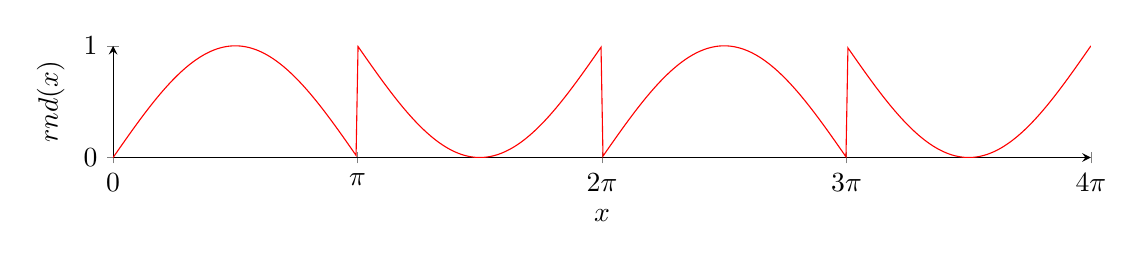
\begin{tikzpicture}[scale=1.0]
        \begin{axis}[
            samples=500,
            domain=0:4*pi,
            axis lines=left,
            xlabel=$x$,
            ylabel={$rnd(x)$},
            height=3cm,
            width=14cm,
            ytick={0,1},
            xtick={0,pi,2*pi,3*pi,4*pi},
            xticklabels={$0$,$\pi$,$2\pi$,$3\pi$,$4\pi$}
            ]
        \addplot[red] plot (\x, { sin(\x*1 r) - floor(sin(\x*1 r)) });
        \end{axis}
    \end{tikzpicture}
    \caption{Random numbers with the fractional value of sine of x.}
\end{figure}

\noindent
The sine values fluctuate between $-1$ and $1$, but with $fract$, only the fractional part is evaluated, turning the negative values in positive ones.
This effect can be used to get some pseudo-random values by "compressing" the function vertically or in other words, by increasing the frequency of the sine wave.
\\
The next figure displays the function $rnd(x) = fract(sin(x) * 10000)$.

\begin{figure}[H]
    \centering
    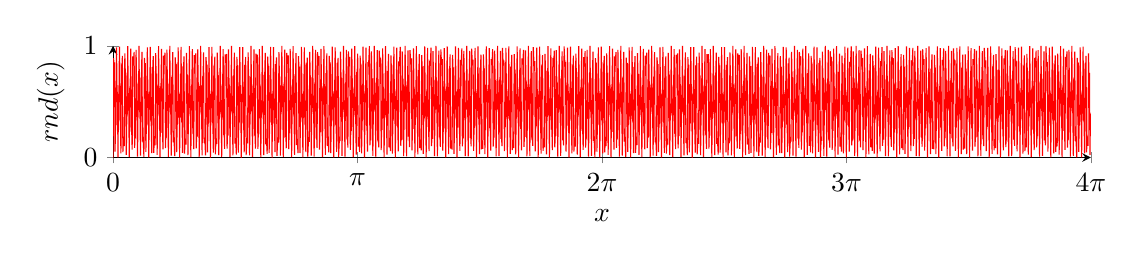
\begin{tikzpicture}[scale=1.0]
        \begin{axis}[
            samples=2000,
            domain=0:4*pi,
            axis lines=left,
            xlabel=$x$,
            ylabel={$rnd(x)$},
            height=3cm,
            width=14cm,
            ytick={0,1},
            xtick={0,pi,2*pi,3*pi,4*pi},
            xticklabels={$0$,$\pi$,$2\pi$,$3\pi$,$4\pi$},
            ]
        \addplot[red] plot (\x, { sin(\x*10000) - floor(sin(\x*10000)) });
        \end{axis}
    \end{tikzpicture}
    \caption{Random numbers with the fractional value of sine of x multiplied by 100000.}
\end{figure}

\noindent
It is clearly visible that the function $rnd(x)$ became chaotic and seemingly random. However, it is noteworthy that $rnd(x)$ is still a deterministic function, which means for example $rnd(1.0)$ is always going to return the same value.